\section{Problem Description}

The goal of the project is to recommend papers to researchers according to their interest. There are two main features to represent users' interest. The first will be keywords. The second will be researcher's reading history.  
%We will also consider other interesting patterns according to experiments.

%We will solve the problem of paper recommendation based on keywords, citation network and user reading history. 
We will have an offline dataset consisting of paper citation relation and papers' content.

Next, we give formal notations to describe our problem. We separate the problem into two part: given the interested keywords then the system output a list of recommending papers, or given a list of read papers in user's history then the system output a list of recommended papers. 

\subsection{First Part: Recommend According to Keywords}

For the first part, the input will be a list of $n$ strings $K = [k_1, k_2, ..., k_n]$, where each string is an interested field, e.g. ["machine learning", "computer vision"]. The desired paper list will be $R = [r_1, r_2, ..., r_m]$, in the form of indexs of $m$ papers. Our system will recommend papers in an ordered way, which means $r_i$ is a better paper than $r_{i+1}, \forall i$.

\subsection{Second Part: Recommend According to Reading History}

For the second part, the input will be a list of papers $P = [p_1, p_2, ..., p_n]$, where each paper is represented as a unique id, e.g. ["journals/cacm/Szalay08"]. This represents user's reading history ignoring the time sequence. The desired paper list will be $R =  [r_1, r_2, ..., r_m]$, in the form of indexs of $m$ papers. Our system will also recommend papers in an ordered way, which means $r_i$ is a better paper than $r_{i+1}, \forall i$.

\subsection{Graph representation}

First of all, we represent the citation relations among papers to be a directed graph $G=(V, E)$. $V$ is the vertex set, each vertex represents a paper, we use the index to represent each paper. We also stored the detailed information of papers in a separated map from index to information. $E$ is the directed edge set. $\exists e=(v -> u) \in E$ means the paper $v$ cites the paper $u$.

\subsubsection{Subgraph}
We also need the concept of subgraph $G_s = (V_s, E_s)$. In the subgraph, we ensure that $V_s \subseteq V$, meaning we keep a subset of the original graph and get rid of the other vertexes. Then we compute the sub-edge set according to the sub-vertexes set: $E_s = \{e=(u -> v) | u \in V_s and v \in V_s\ and e \in E\}$. In this work, we do not need other subgraphs, which means a subgraph is determined by the original graph $G$ and the sub-vertexes set $V_s$.

\subsubsection{Reverse Graph}
Since we are working on a directed graph, we can define the concept of a reversed graph. $G^*=(V^*, E^*)$ is a reversed graph of $G=(V, E)\iff $
\begin{equation}
 V^* = V \text{, and } E^* = \{(u -> v)| (v->u) \in E\}.
\end{equation}

\subsubsection{Patterns}

According to previous network studies {TODO, related work about patterns}, several common patterns are extremely useful for recommendation on networks. We address two main patterns: the diamond pattern and the triangle pattern. 

\paragraph{Diamond pattern}

\begin{figure}[t]
	\centering
	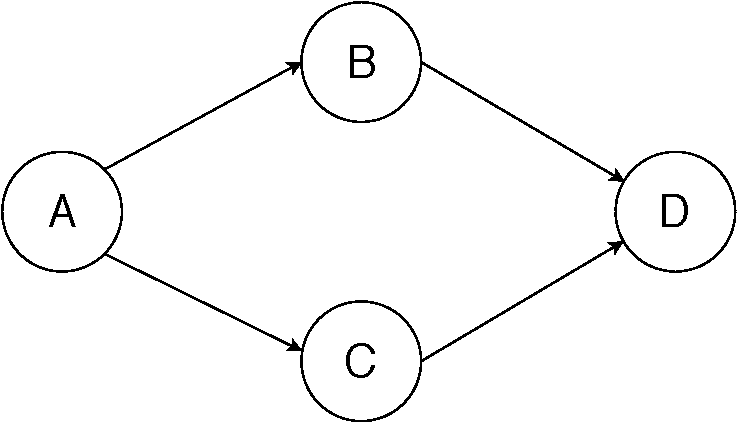
\includegraphics[width=0.7\linewidth]{diamond.pdf}
	\caption{Example of a diamond pattern.}
	\label{fig:diamond}
\end{figure}

As shown in Figure \ref{fig:diamond}, a diamond pattern is that if a user has read paper $A$, and paper $A$ cites both paper $B$ and $C$, paper $B$ and $C$ both cite paper $D$. Then, we will recommend paper $D$ to the user if the paper has not been read. This is easy to understand because paper $D$ may be an important work in the reader's interested field.

\paragraph{Triangle pattern}

\begin{figure}[t]
	\centering
	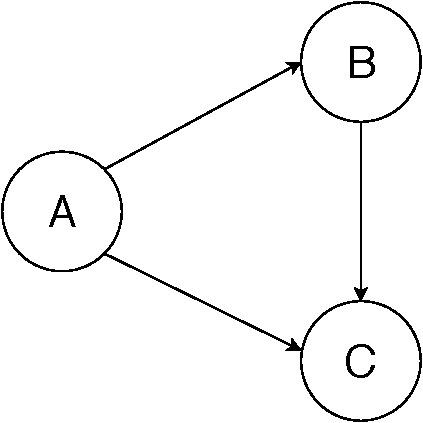
\includegraphics[width=0.7\linewidth]{triangle}
	\caption{Example of a triangle pattern.}
	\label{fig:triangle}
\end{figure}

Triangle is also easy to understand. As shown in Figure \ref{fig:triangle}, a triangle pattern is that if a user has read paper $A$, and paper $A$ cites both paper $B$ and $C$, paper $B$ cites paper $C$. Then, we will recommend paper $C$ to the user if the paper has not been read. 

